\RequirePackage{plautopatch}
\RequirePackage[l2tabu, orthodox]{nag}

\documentclass[platex,dvipdfmx]{jlreq}			% for platex
% \documentclass[uplatex,dvipdfmx]{jlreq}		% for uplatex
\usepackage{graphicx}
\usepackage{bxtexlogo}
\usepackage{url}
\pagestyle{empty}

\title{身体動作による創作・演奏ウェブアプリ\\
《音たっちくん》の制作と音遊びの応用}

\author{
国立音楽大学演奏・創作学科コンピュータ音楽専修\\
藤井 久隆 上原 彩愛 印南 智樹 濱野 峻行
}
\date{}

\begin{document}
\maketitle

\section*{概要}
中高生を対象としたデジタルメディアによる音楽創作・演奏体験にはより一層の多様性が求められる中、ウェブテクノロジーや身体動作に関する技術の活用は当該対象を含め幅広いユーザに対して音楽的インタラクションを形成しうるものになる。\cite{kakaku}本研究では発表者らの共創開発チームにより、ウェブブラウザで遊ぶことのできるサウンドアプリケーション《音たっちくん》(おんたっちくん)を制作した。このアプリはウェブベースでTensorFlow.jsによる身体動作検出のための学習済みモデルを採用しており、ユーザは音素材を画面上に配置し、カメラに向かって指をかざして演奏することができる。アプリの特徴には直感性・手軽さ、身体動作との同期による演奏感、創意工夫の自由度・協同性などが挙げられる。これらの観点に基づき、実際に高校生を対象として行った協同創作ワークショップで見られた創発的な知見も含め、本アプリへの評価として音遊びの応用提案を行う。

% imgImportTemplate
% \begin{figure}
% \centering
% \includegraphics[width=70mm]{figures/Sample.png}
% \caption{ここにキャプションを挿入します}
% \label{fig:model}
% \end{figure}

\section{制作背景}
\subsection{現状課題}
世界的なSTEAM教育の高まりによって、タブレット型の端末などを使用した授業形式が普及してきている。そのため、メディアの強みを活かした教育アプリケーションと各教科の連携が求められている。音楽科目に着目したとき、現時点で以下のような課題があることを発見した。
\begin{itemize}
  \item ICT教育の進展に伴う普及の不均衡:現状ではICT教育が進んでいるが、音楽教育においてはアプリケーションの利用が他の科目に比べて少ない。
  \item 音楽教育のデジタル化の遅れ:音楽教育において、演奏や創作に関連するアプリケーションの不足があり、音楽初学者にとって手軽に使うことのできるものが少ない。
  \item 楽器演奏と創作への心理的ハードル:西洋音楽の規範に基づく楽譜による演奏や創作において、評価基準が厳しく、生徒に上手・下手の意識や心理的ハードルを生む。
  \item デジタルツールの複雑さと理解の障壁:DTMなどの音楽創作ソフトの利用において、コンピュータに不慣れな人が直面する複雑なインストールや操作、記譜法の理解の障壁が存在する。
\end{itemize}
これらの課題は音楽科目特有の原因があるため、音楽分野からの解決アプローチが求められると考えた。

\subsection{解決策の提案}
上記の課題を解決するために、以下の4点のアイデアを目標にした音楽教育アプリケーションの開発に取り組んだ。
\begin{itemize}
  \item 普遍的なアプリケーションの開発:音楽の習得度に関係なく利用できるアプリケーションの開発を検討し、これを通じて音楽教育のデジタル化を促進する。
  \item 身体性を活かしたアプローチ:身体性を軸に据え、生得的な知識を活かすアプローチを採用し、例えばキネクトを用いた身体演奏のようなアイデアを導入することで、演奏や創作の手法において生徒が自然に取り組める環境を整える。
  \item 新しい音楽体験の提供:音楽の楽しさや興味を引き出すため、楽器から離れた音色や見た目、演奏方法に焦点を当て、中学生や高校生にとっても実践しやすいアプローチを検討する。
  \item 包括的な音楽教育プログラムの構築:西洋音楽の知識に依存せず、包括的かつ多様な音楽教育プログラムを構築し、生徒が柔軟かつ自由に音楽を楽しめる環境を整える。
\end{itemize}
そして実際に高校生の音楽の授業で作成したアプリケーションを使用していただき、フィードバックを得ることで評価と考察をすることを目的とした。

\section{アプリケーション内容}
\subsection{音たっちくんの遊び方}
GoogleChromeを開き、音たっちくんのリンク(https://st.kcm-sd.ac.jp/public/ontouch/)を入力することで起動することができ、タイトルページのスタートボタンを押すことで以下のような操作画面が表示される。
\newpage

\begin{figure}
\centering
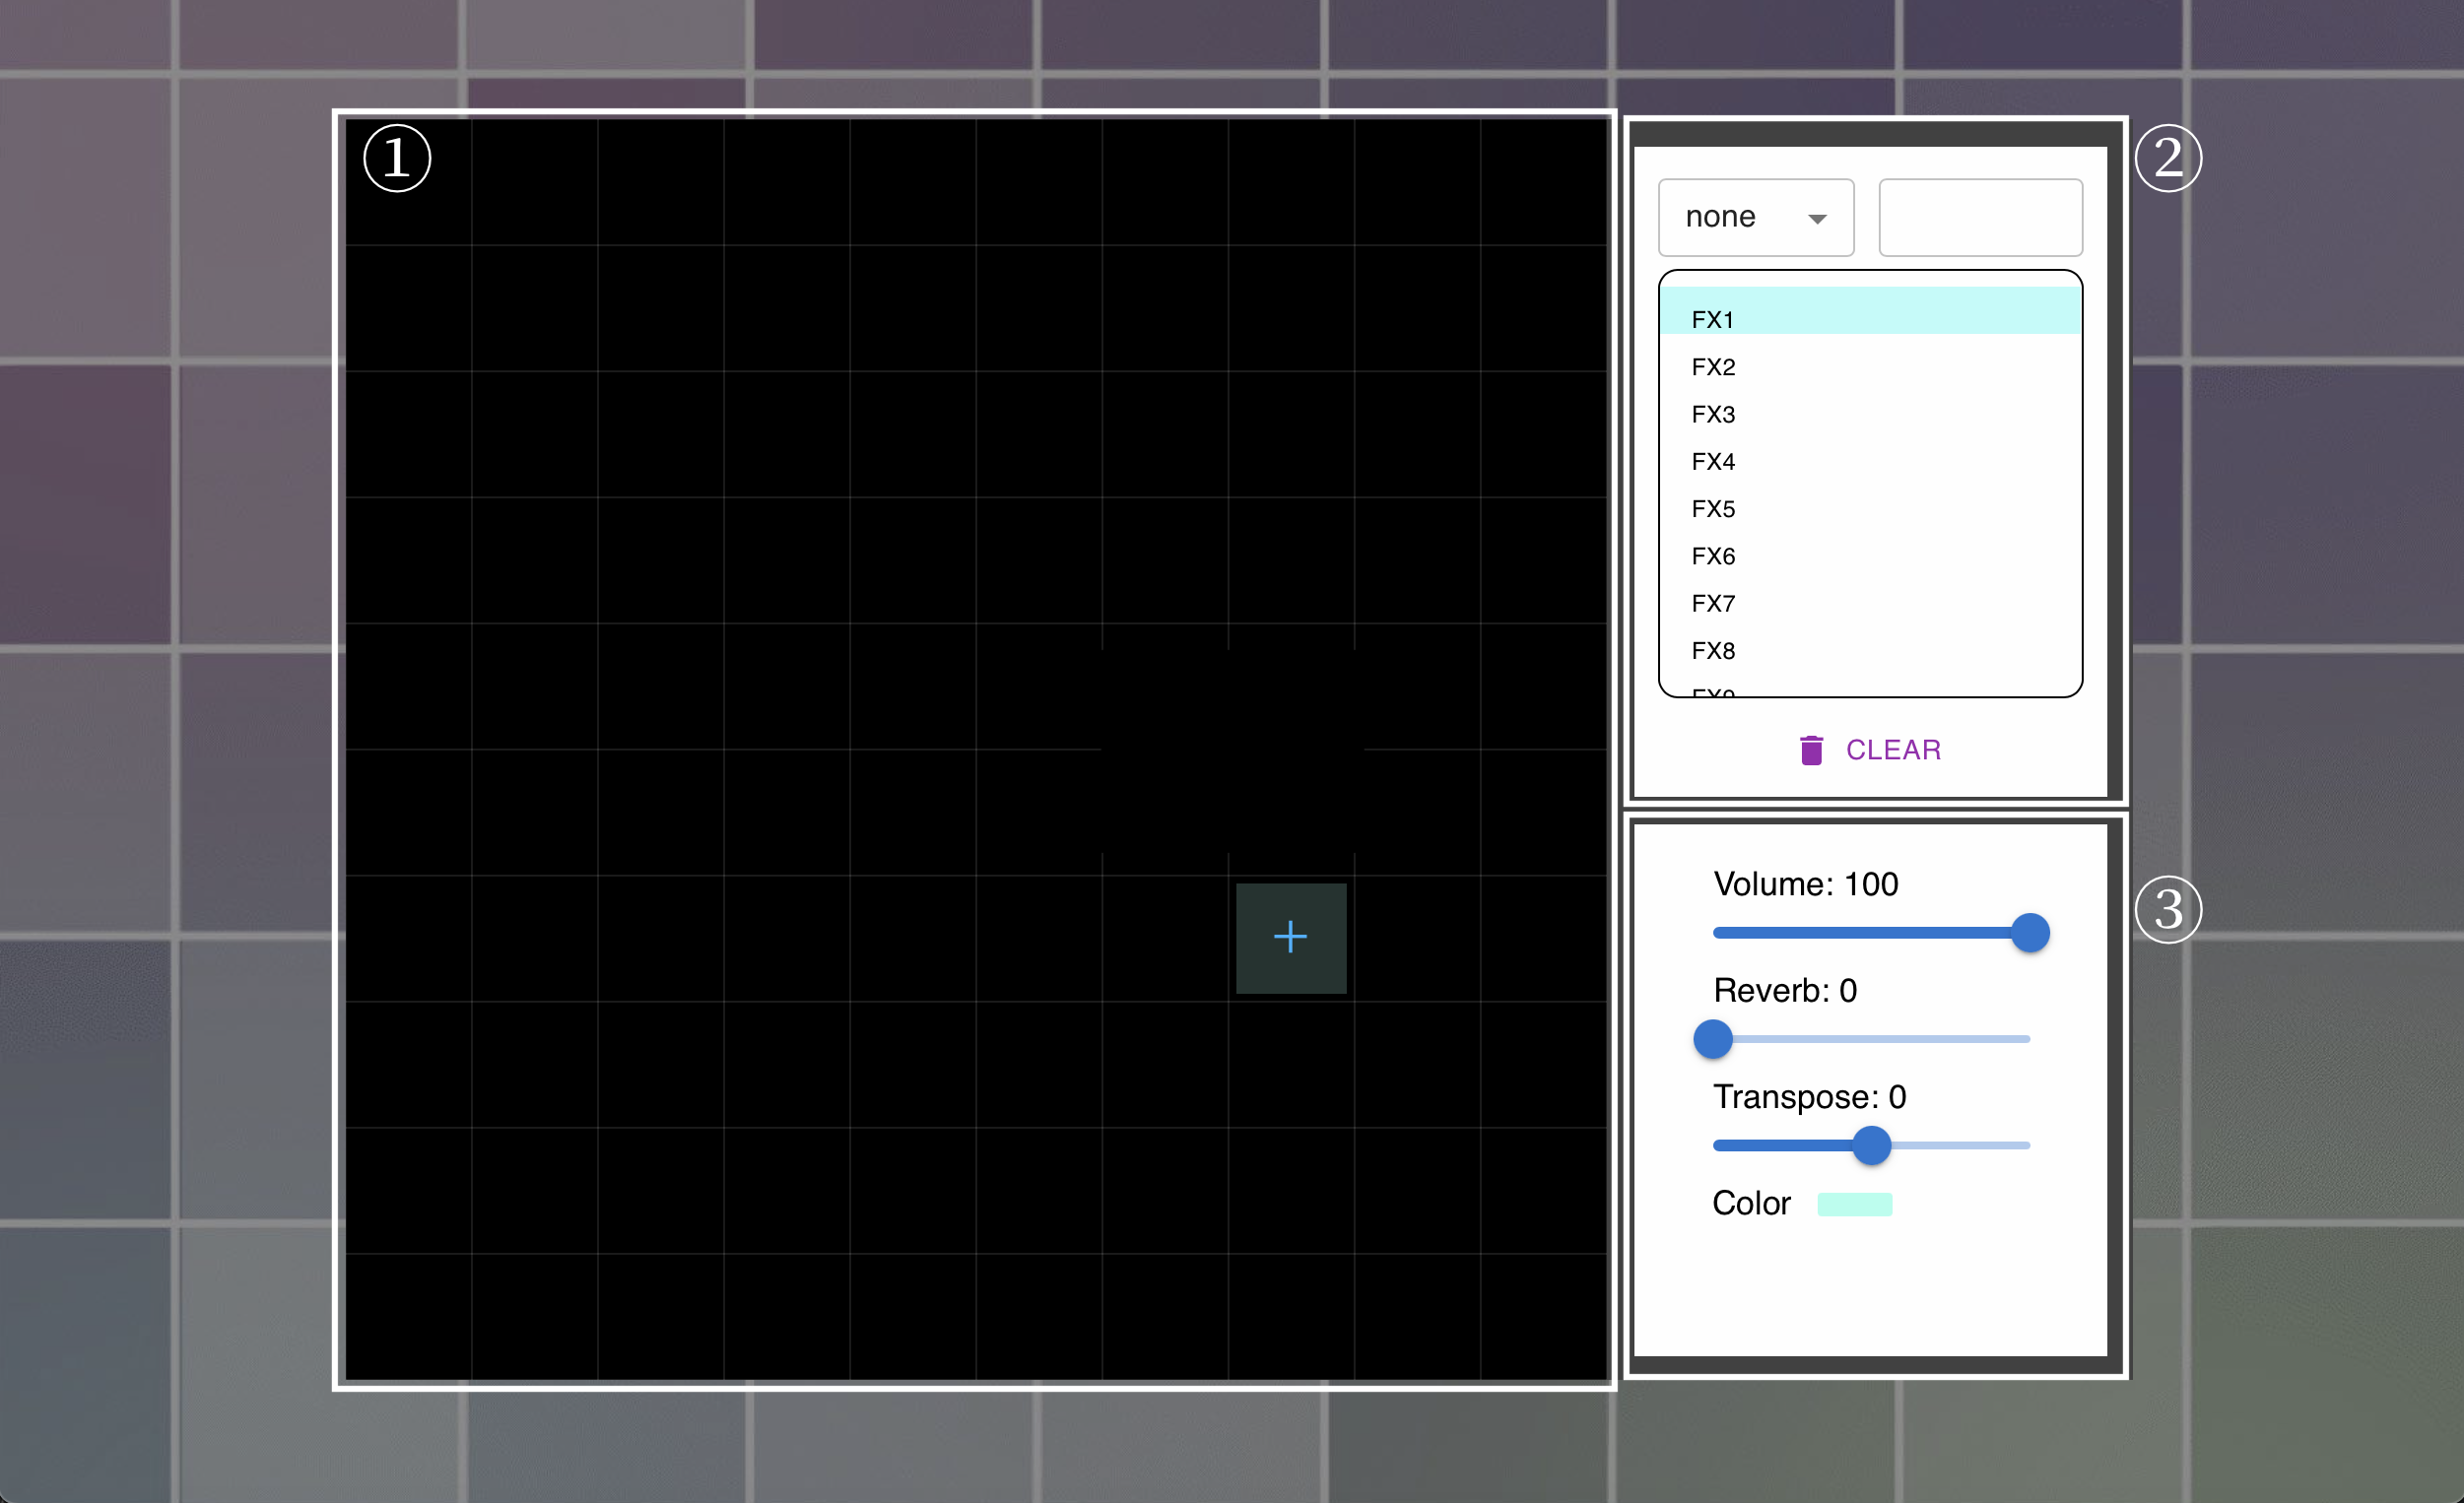
\includegraphics[width=100mm]{figures/onTouch_screenShots1.png}
\caption{音たっちくんスクリーンショット(仮)}
\label{fig:model}
\end{figure}

操作画面は大きく分けてグリッド画面、音選択画面、調整画面の3つに分かれている。それぞれがどのような役割を持っているのかを説明していく。
\begin{enumerate}
  \item グリッド画面:画面左側にあるカメラの映像の上に10×10のグリッドが重なっている画面、これがグリッド画面である。音を配置したいグリッドを選択すると十字のカーソルが表示され、そのグリッドでの音制作を開始することができる。
  \item 音選択画面:画面右上側にある画面の「FX1」などの項目を選択すると、グリッド画面で選択中のグリッドに音源を設定することができる。環境音や声など多種多様な音源が用意されており、音探しを行うのに役立つのが絞り込みツールと検索ツールである。音選択画面左上の四角をクリックすると、音源それぞれのジャンルごとに絞り込むことができ、右上の四角にテキストを入力すると音源名で検索をかけることができる。
  \item 調整画面:画面右下側にある画面のパラメータを動かすと、手を翳した時のグリッドの音や見た目の様々な設定をすることができる。音の調整にはVolume、Reverb、Transposeの3つのスライダーが用意されている。
  \begin{itemize}
    \item Volume:Volumeのスライダーを調整すると、音量を調整することができる。0~100で調整が可能であり、0は無音、100は最大音量である。
    \item Reverb:Reverbのスライダーを調整すると、残響の量を調整することができる。0~100で調整が可能であり、0は残響なし、100は最大の量である。
    \item Transpose:Transposeのスライダーを調整すると、音のピッチの高さと速度を調整することができる。デフォルトが0となっており、-12(1オクターブ下)~12(1オクターブ上)の範囲で調整が可能である。
  \end{itemize}
  スライダーの下にあるColorをクリックし、好みの色を選択するとデフォルトで水色となっているグリッドの色を設定することができる。
\end{enumerate}

\subsection{システム解説}
音たっちくんでは、指の座標を取るためにTensorflow.jsを使用した。Tensorflow.jsとは、ブラウザ上で機械学習の機能を使うためのJavaScriptライブラリである。カメラの入力に対してTensorflow.jsを使用し、取得した手の指や関節などの座標から人差し指の座標のみを使用し、円が追従するようにした。音声においてはWebAudioAPIを使用している。

\section{実践と遊び方の発見}
\subsection{高校生向けワークショップの開催}
作成した音たっちくんを高校生に体験していただいた。音楽の授業の一環として、ワークショップ形式で行われた。サウンドスケープ制作という内容でチームごとにサウンドスケープ(音風景)を構築する形式を採用した。作成したワークシートのガイドラインに基づき、参加者は音の空間のコンセプトを考え、選択した音の素材と構成を使ってグループ内で協力してサウンドスケープを制作する。同時に、演奏の時間の使い方や動きの工夫について考え、実際に音を出しながら、体を動かしながら制作していただいた。ワークショップの最後には、グループが制作したサウンドスケープを元に、全身を使ったパフォーマンスを発表し、他のチームのパフォーマンスも鑑賞した。

\subsection{得られた発見}
実際にワークショップをしていただいた中で、2つの発見を得ることができた。1つ目は制作側の意図しないパフォーマンス工夫だ。演奏するカメラを向かい合わせにすることで演奏の見せ方を工夫したり、パネルの色や配置で絵を書くなど、参加者が自らアイデアを出し合いながら新しい演出を試みた。これらの中には制作時には予想されていなかった表現方法もあり非常に興味深い結果となった。2つ目は音楽制作の楽しさと遊びの共通性だ。参加者が楽しそうに交流し、ユニークな演奏アイデアを生み出したことから、音たっちくんの設計要素と音楽創作の楽しさ、遊びの要素に共通性がある可能性が浮かび上がった。高校生たちが自由にアプローチできる環境を提供することで、音楽創作における楽しさや遊び方が広がることが示唆された。


\section{音たっちくんの遊び方考察}
ワークショップから得られた具体的な遊びかたをもとに、遊び方の発想を以下の4つに分類した。
\begin{itemize}
  \item 共創的発想:ストーリー分担(時間セクションで分担、or パートで分担)、2,3人で動き連携、複数台利用 or 1台で3人同時演奏
  \item 動きの発想:指で繊細な演奏、タイミングのコントロール、指 or 全身
  \item 絵的な発想:パネルの配置で絵を描く、色
  \item 音楽的発想:絶対音楽と標題音楽 時間構成
\end{itemize}
これらの発想が生まれた要素として以下の3点が考えられる。1つ目は身体的なフィードバックがあることだ。楽器の演奏に必要な身体的な技術が不要であるため、音たっちくんでは音と身体がより連携しやすくなり、より自由な動きのアイデアが生まれたと考えられる。2つ目は音素材の多様性だ。ジャンルにとらわれない音素材の導入により、身近な音素材と異なる音を組み合わせ、新しいストーリーやコンセプトを生み出す契機となった。普段聞き慣れないシンセサイザーや効果音のような音素材も実験的な発想を引き出す助けとなったと考えられる。3つ目は音楽知識の有無によるアプローチ方法の多様性だ。音楽の知識を持っていることで音階やハーモニー、リズムといった表現への挑戦が可能になる。音楽知識のバックグラウンドに関わらず、体験者の持っている考え方を活かせるものとなった。

\section{課題と今後の提案}
(メモ)ここに今後の課題についてのテキストが入ります。

\begin{thebibliography}{99}

\bibitem{kakaku}
(メモ)参考文献テストテキスト

\end{thebibliography}




\end{document}

